\newpage

\section{Неделя V}


\subsection*{№1}

Найдём функцию Грина оператора $\partial_x^2 (\partial_x^2 + 1)$ для функций над $[-\pi, \pi]$, удовлетворяющих граничным условиям. 

Подстановкой $e^{\lambda x}$, найдём, что нулевые моды удовлетворяют уравнению
\begin{equation*}
    \lambda^2 (\lambda - i)(\lambda + i) = 0,
    \hspace{0.5cm} \Rightarrow \hspace{0.5cm}
    e_{1, 2, 3} = \frac{1}{2\pi} \left\{1,\,  e^{ix},\,  e^{-ix}\right\},
\end{equation*}
где $2 \pi$ -- нормировка. 

Тогда функция Грина удовлетвоярет уравнению, вида
\begin{equation*}
    \hat{L} G(x) = \delta(x) - \frac{1 + 2 \cos x}{2\pi}.
\end{equation*}
При $x > 0$ общее решение может быть найдено в виде
\begin{equation*}
    G^{\text{gen}}(x) = -c_1 \cos x - c_2 \sin x + c_3 + x c_4.
\end{equation*}
Частное решение:
\begin{equation*}
    G^{\text{part}}(x) = -\frac{x^2}{4\pi} + \frac{4 \cos x}{2\pi} + \frac{x \sin x}{2\pi}.
\end{equation*}
Вклад от $\delta(x)$ можно записать, как
\begin{equation*}
    G^{\delta}(x) = \theta[x] (x -\sin x).
\end{equation*}
Осталось подставить граничные условия , откуда находим:
\begin{equation*}
    G(\pi) = G(-\pi),
    \hspace{0.5cm} \Rightarrow \hspace{0.5cm}
    1 + 2 c_4 = 0.
\end{equation*}
Остальные граничные условия на $G',\, G'',\, G'''$ выполняются автоматически. 

Однако по постановке задачи $G(x)$ не содержит $e_{1,\, 2,\, 3}$, а значит
\begin{equation*}
    \left\{\begin{aligned}
        \langle e_1 | G(x) \rangle &= 0,
        \hspace{0.5cm} \phantom{\Rightarrow} \hspace{0.5cm}
        \pi (\pi + 6 c_3) = 3 \\
        \langle e_2 | G(x) \rangle &= 0,
        \hspace{0.5cm} \Rightarrow \hspace{0.5cm}
        \pi(2 i + 4 c_1 + 4 i c_2) =1, \\
        \langle e_3 | G(x) \rangle &= 0,
        \hspace{0.5cm} \phantom{\Rightarrow} \hspace{0.5cm}
        4 \pi c_1 - 2 i \pi  - 4 i \pi c_2 = 1.
    \end{aligned}\right.
    \hspace{0.5cm} \Rightarrow \hspace{0.5cm}
    \left\{\begin{aligned}
        c_1 &= 1/4\pi, \\
        c_2 &= -1/2, \\
        c_3 &= (3-\pi^2)/6 \pi. \\
    \end{aligned}\right.
\end{equation*}
Таким образом, искомая функция Грина:
\begin{equation*}
   G(x) =  (\theta[x] - \tfrac{1}{2}) (x - \sin x) 
    -\frac{x^2}{4\pi} + \frac{5 \cos x}{4\pi} + \frac{x \sin x}{2\pi} + \frac{1}{2\pi}-\frac{\pi}{6}.
\end{equation*}


\subsection*{№1 (пример)}


Рассмотрим, например, возмущение, вида
\begin{equation*}
    \varphi(x) = \sign(x) \cos (x).
\end{equation*}
Стоит заметить, что $\varphi(x)$ не содержит в себе нулевых мод, так что задача корректна и имеет решение. 
Уже зная $G(x)$ для $\hat{L}$, нетрудно найти решение:
\begin{equation*}
    f(x) = \int_{-\pi}^{\pi} G(x-y) \varphi(y) \d y = 
    -\theta (x) (x \sin (x)+2 \cos (x)-2)+\frac{(2 x+\pi ) (\pi  \sin (x)-4)}{4 \pi }+\cos (x).
\end{equation*}
Посмотрим на вид $G(x),\, f(x)$ и также для наглядности построим все слагаемые $f(x)$, а то как-то больно хорошо $f(x)$ выглядит.
\begin{figure}[ht]
    \centering
    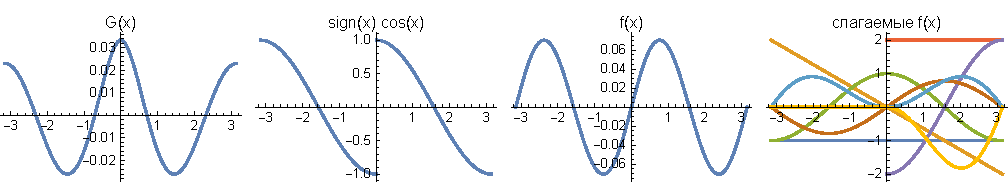
\includegraphics[width=0.9\textwidth]{figures/w5_1.pdf}
    \caption{Вид функций в w5, №1.}
    %\label{fig:}
\end{figure}


\subsection*{№2 (2.2.3)}


Переёдем в сферические координаты для интеграла, вида
\begin{equation*}
    f(\vc{r}) = \int G(\vc{r} - \vc{r}') \phi(\vc{r}') \d V',
    \hspace{5 mm} 
    G(\vc{r}) \equiv G(r) = - \frac{1}{4 \pi r},
    \hspace{0.5cm} \Rightarrow \hspace{0.5cm}
    f(\vc{r}) = - \int dV'\ \frac{\phi(\vc{r}')}{4 \pi |\vc{r}-\vc{r}'|}.
\end{equation*}
Считая, что $\phi(\vc{r}) \equiv \phi(r)$, находим:
\begin{equation*}
    f(\vc{r}) = \frac{1}{r} \int_0^r \phi(r') r'^2 \d r' + \int_r^\infty \phi (r') r' \d r'.
     % = - \int_0^{\pi} \sin \theta \d \theta \int_{0}^{2\pi} \d \varphi \int_0^{\infty}
    % \frac{\phi(r) r^2 }{2 \pi |\vc{r}-\vc{r}'|}
    % \d r  = - \int
\end{equation*}







\subsection*{№3 (2.2.10)}

Найдём решение уравнения Лапласа $f$ в полуплоскости $y > 0$, для $f(x, 0) = e^{ix}$. Искомая функция может быть найдена, как
\begin{equation*}
    f(x, y) = \int_{\mathbb{R}} \frac{y/\pi}{(x-\xi)^2 + y^2} e^{i \xi}.
\end{equation*}
У подынтегральной функции всего две особенности: $\xi = x \pm i y$ -- полюса первого порядка. По лемме Жордана, замыкая функцию сверху, интегрируя против часовой стрелки, находим значение интеграла через вычет в точке $x + i y$:
\begin{equation*}
    f(x, y) = 2 \pi i \frac{y}{p} \lim_{\xi \to x + i y} \frac{(\xi-x-iy)}{(x-\xi)^2 + y^2} e^{i \xi} = e^{i x - y},
\end{equation*}
таким образом нашли голоморфную функцию, удовлетворяющую граничному условию.








\subsection*{№4 (2.3.2)}

Найдём радиальную функцию $R$ связного состояния атома водорода, соответствующего $n=2$ и $l=1$. 


Вообще, волновая функция для атома водорода будет иметь вид
\begin{equation*}
    \psi _{nlm}(r,\theta ,\varphi )=\sqrt {\frac {(n-l-1)!}{2n{\cdot }(n+l)!}}{\cdot }\left({\frac{2}{n}}\right)^{\frac{3}{2}}\cdot \exp {\left({-{\frac{r}{n}}}\right)}\cdot \left({\frac {2r}{n}}\right)^{l}L_{n-l-1}^{2l+1}{\left({\frac {2r}{n}}\right)}\cdot Y_{l,m}(\theta ,\varphi ),
\end{equation*}
где $L$ -- полиномы Лагерра. Так что ожидаем найти, что $R \sim r \cdot e^{-r/2}$. 


Образ функции $\Phi = R \cdot r^{l+1}$, может быть записан, как
\begin{equation*}
    \tilde{\Phi} (p) \sim \frac{(p-1/n)^{n-l-1}}{(p+1/n)^{n+l+1}} = \frac{1}{(p+\frac{1}{2})^4}.
\end{equation*}
Делая замену $p = i \nu$, переходим к интегралу
\begin{equation*}
    \Phi(r) = \int_{-\infty}^{+\infty} 
    e^{i \nu t} \frac{1}{(i \nu + \tfrac{1}{2})^4}
    \frac{\d \nu}{2\pi},
\end{equation*}
с полюсом 4 порядка в $\nu = i/2$. Тогда, считая вычет в этой точке, находим
\begin{equation*}
    \Phi(r) = i \lim_{\nu \to i/2} \frac{d^4}{d x^4}  \left(
        \nu - \frac{1}{2}i
    \right)^4 \frac{e^{i \nu r}}{(i \nu - \tfrac{1}{2})^4} = r^3 e^{-r/2},
    \hspace{0.5cm} \Rightarrow \hspace{0.5cm}
    R = r \cdot e^{-r/2},
\end{equation*}
как и ожидалось. Если бы нам хотелось иметь нормированную $R(r)$, то
\begin{equation*}
    \int_{0}^{\infty} r e^{-r/2} \d r = 2 \int_{0}^{\infty} e^{-r/2} \d r = 4,
    \hspace{0.5cm} \Rightarrow \hspace{0.5cm}
    R^{\text{norm}} = \frac{r}{4} e^{-r/2}.
\end{equation*}





